\chapter{Simulation Results and Discussion}
\thispagestyle{fancy}

\section{Fractals}
As discussed in section \ref{sec:CAandSOC}, in order to show that a dynamical system exhibits SOC, some fractal nature must be present. As done analytically for a 1-D-model in \cite{fractal_avalanching}, we can plot the energy of a system over time according to the definition of normalized energy
\[
E(t) = \int_f h(x,y,t)^2 df
\]
where $h$ is the height of a site at position $(x,y)$ of the field $f$ at time $t$. In MATLAB/Octave, at the end of every main loop iteration the energy is calculated:
\begin{lstlisting}
ee(t) = sum(sum(f.^2));
\end{lstlisting}
As the energy series in 1-dimensional case shows fractal properties (see \cite{fractal_avalanching}), the question arises if this is true for a 2-dimensional case.

\section{Power-law distributions}

In this section, we investigate tha avalanche size and lifetime distribution, 
according to different boundary conditions, namely the periodic boundary conditions and open boundary conditions.



\section{Power-law distributions}

In this section, we investigate tha avalanche size and lifetime distribution, 
according to different boundary conditions, namely the periodic boundary conditions and open boundary conditions.



\subsection{Periodic boundary conditions}

For periodic boundary conditions, there is never grain lost if we do not introduce friction. 
This means that, in order to study them, we need to be careful with lattice size and driving time, 
in order to not have all the sites overcritical, which will logically imply never-ending avalanches.
As we  also need good statistics to judge the distribution, we must use a reasonably large lattice, 
though in theory, the lattice is infinite large which would imply the size should not matter.

We studied a $100\times 100$ lattice with a driving time $T=5000$, and the results are presented in the figure~\ref{sp}, 
where we see quite a nice power-law behaviour for avalanche size, but a worse one for the lifetime. 


\begin{figure} 
\begin{center}
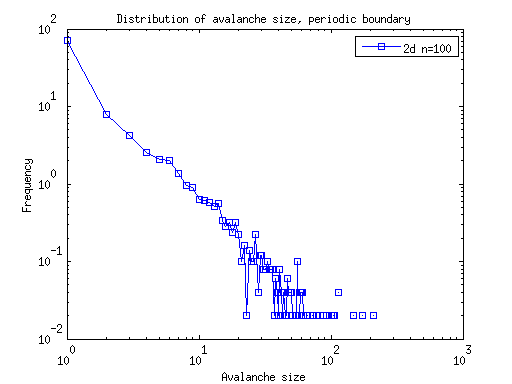
\includegraphics[width=0.49\textwidth]{results/sp.png}
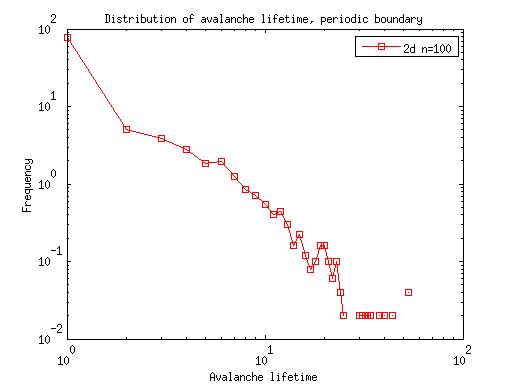
\includegraphics[width=0.49\textwidth]{results/tp.png} 
\caption{Avalanche size and lifetime distribution for $100\times100$ lattice, with periodic boundary conditions. 
The driving time is $T=5000$.  }
\label{sp}
\end{center}
\end{figure} 

Due to memory-demanding large lattices and large driving time, we will not treat higher dimensions.
The periodic boundary case without grain lost, though, is not of much interest, as real systems are finite and dissipative, 
hence, we might not include it as a SOC phenomenon. 

Instead, we should introduce a friction parameter, and hence, consider a \emph{real} $E$ field, in contrast to a discrete integer field. 
The periodic boundary in principle implies lattice size independence, which will represent a computational advantage, as we can choose small lattice.
Indeed, this is true, however, the driving time whould increase with size in order to get enough statistics. 

We studied this situation for $d=2$, with $n=10$, $n=50$ and $n=100$. See figure~\ref{spf} for the results. 
We see a clear cut-off for large avalanche number due to friction, though the we have a quite nice power-law distribution for small avalanches.
The lifetime is not shown, as it shows worse statistics, which do not differ too much from the case in figure~\ref{sp}.

Besides, we can be more or less secure to use small lattices with also smaller total driving time, therefore, 
this criteria will be used to explore higher dimensional lattices.
Figure~\ref{dsp} shows some plots. The cut-off effect due to friction is much less than the $2d$ lattice, 
but we can increase it and check again the effect of friction (see figure~\ref{3spf}).
From this analysis, clearly, the dissipation plays an important role, nevertheless, on \emph{average}, 
the total energy of lattice is kept constant when the system evolves, see figure~\ref{ep}. 

Furthermore, for $d=1$, we clearly do not see critical behaviour, in agreement with the prediction of theory (the situation for open boundary is also checked to be the same). Figure~\ref{1p}. 

\begin{figure} 
\begin{center}
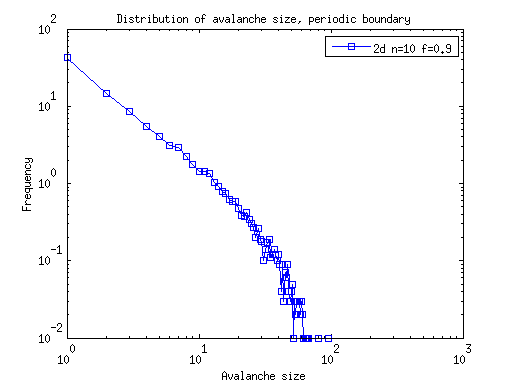
\includegraphics[width=0.49\textwidth]{results/spf.png}
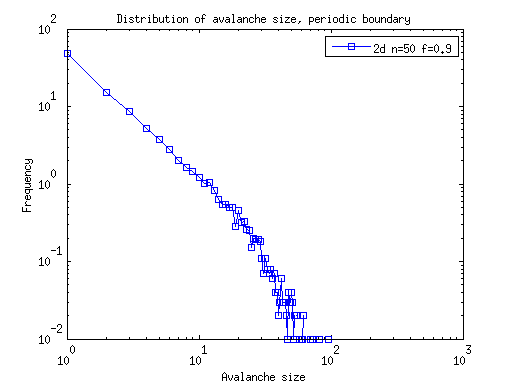
\includegraphics[width=0.49\textwidth]{results/spf50.png} \\
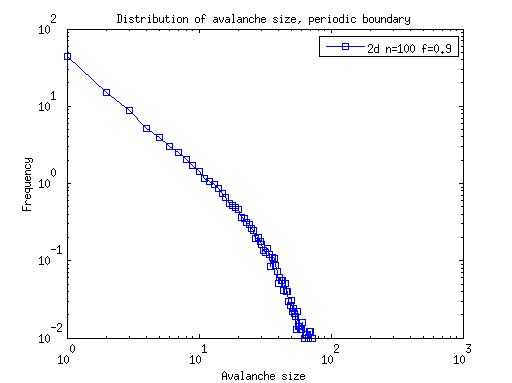
\includegraphics[width=0.49\textwidth]{results/spf100.png} 
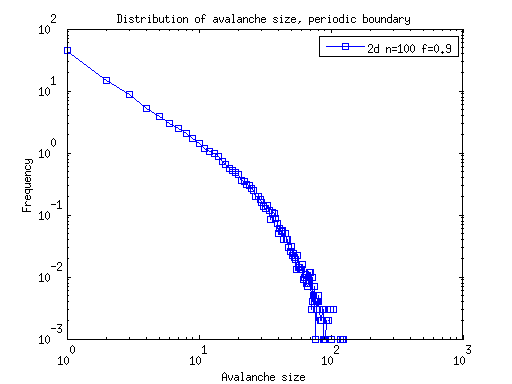
\includegraphics[width=0.49\textwidth]{results/spf100a.png}
\caption{Avalanche size distribution for $2d$ lattice with friction, with periodic boundary conditions. 
The driving time is $T=10000$ for $n=10$ and $n=50$, and $T=100000$ for $n=100$. 
This latter case is showed first the restricted axis for a good comparison and the complete statistics, from which we see a clear cut-off due to friction.  }
\label{spf}
\end{center}
\end{figure} 



\begin{figure} 
\begin{center}
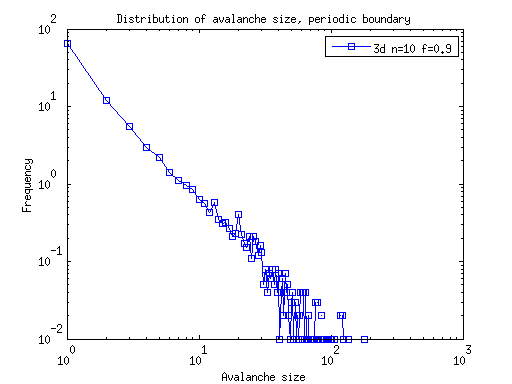
\includegraphics[width=0.49\textwidth]{results/3spf.png}
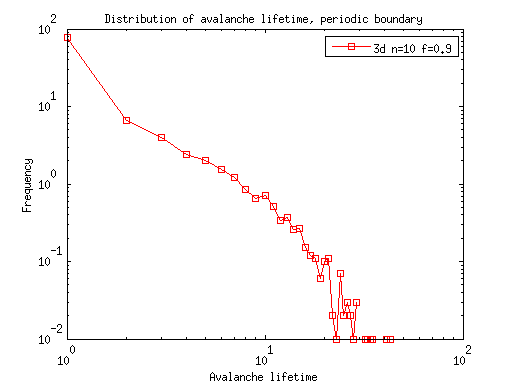
\includegraphics[width=0.49\textwidth]{results/3tpf.png} \\
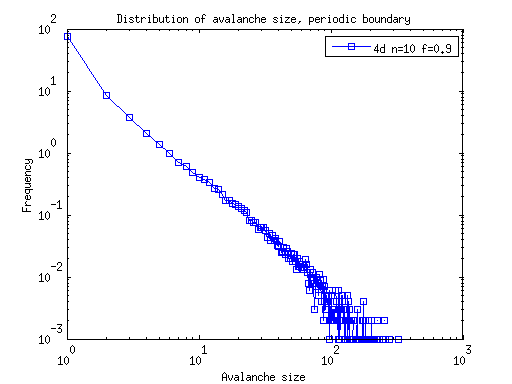
\includegraphics[width=0.49\textwidth]{results/4spf.png}
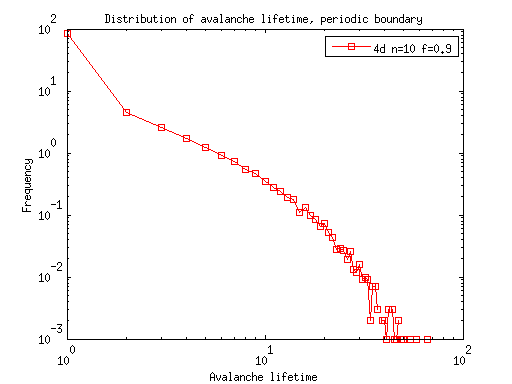
\includegraphics[width=0.49\textwidth]{results/4tpf.png} 
\caption{Avalanche size and lifetime distribution for $3d$ and $4d$ lattices with friction and periodic boundary conditions. }
\label{dspf}
\end{center}
\end{figure}  


\begin{figure} 
\begin{center}
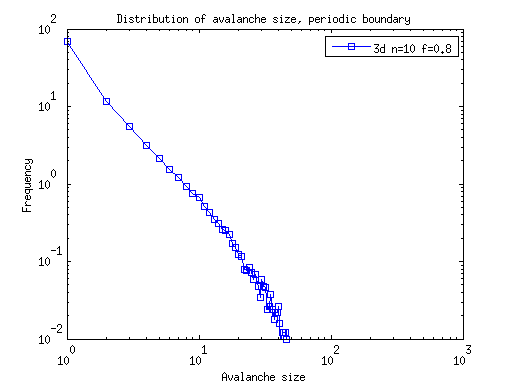
\includegraphics[width=0.49\textwidth]{results/3spf08.png}
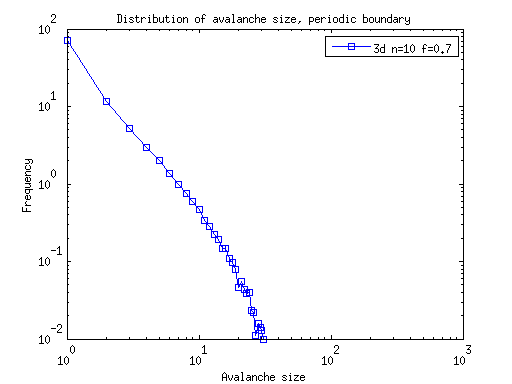
\includegraphics[width=0.49\textwidth]{results/3spf07.png} 
\caption{Avalanche size distribution for $3d$ lattice with different friction parameter and periodic boundary conditions. }
\label{3spf}
\end{center}
\end{figure}  

\begin{figure} 
\begin{center}
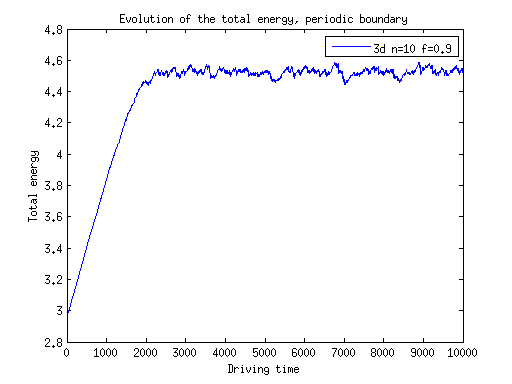
\includegraphics[width=0.49\textwidth]{results/3ep.png}
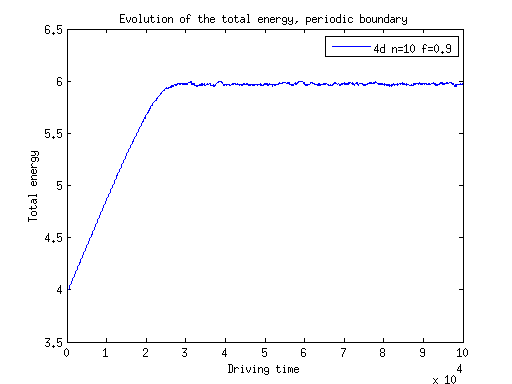
\includegraphics[width=0.49\textwidth]{results/4ep.png} 
\caption{Normalized total energy evolution for $3d$ and $4d$ lattices with friction and periodic boundary conditions. }
\label{ep}
\end{center}
\end{figure}  




\begin{figure} 
\begin{center}
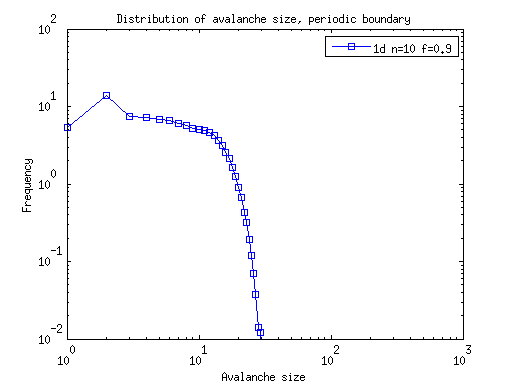
\includegraphics[width=0.49\textwidth]{results/1sp.png}
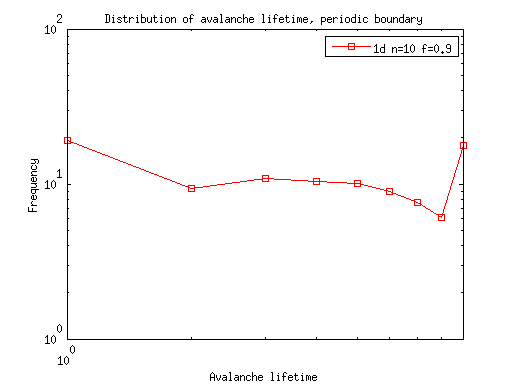
\includegraphics[width=0.49\textwidth]{results/1tp.png} 
\caption{Avalanche size and lifetime distribution for $1d$ lattices with friction and periodic boundary conditions and $T=10^5$. There is no criticality for this case. }
\label{1p}
\end{center}
\end{figure} 










\subsection{Finite boundary conditions}

For the finite boundaries, we have a automatic mechanism to drop the added grains during the driving time, however, unlike the previous case, we have to deal with finite size effects. 

A perturbation in the boundary might give a different avalanche distribution than a perturbation placed in the bulk,
as one might expect that bulk perturbation to produce bigger avalanches, 
because the grain has to be transported further in order to be lost in the boundaries.

We study this effect for 2-dimensional case, and remarkably, we do see different avalanche size distributions (figure~\ref{sv}). 
Furthermore, the high dispersion in large avalanche sizes for the bulk case causes a worse power-law distribution compared to the boundary perturbation case.

For a randomized perturbation sites, the result approaches more to the bulk one. 
\begin{figure} 
\begin{center}
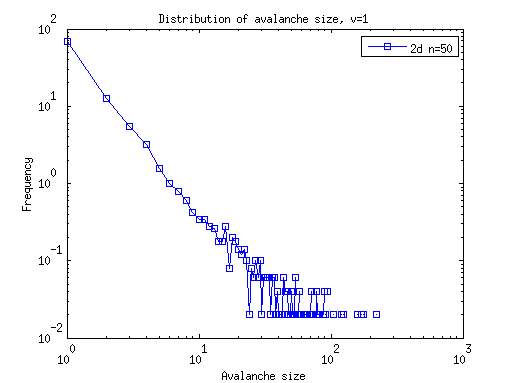
\includegraphics[width=0.49\textwidth]{results/sv1.png}
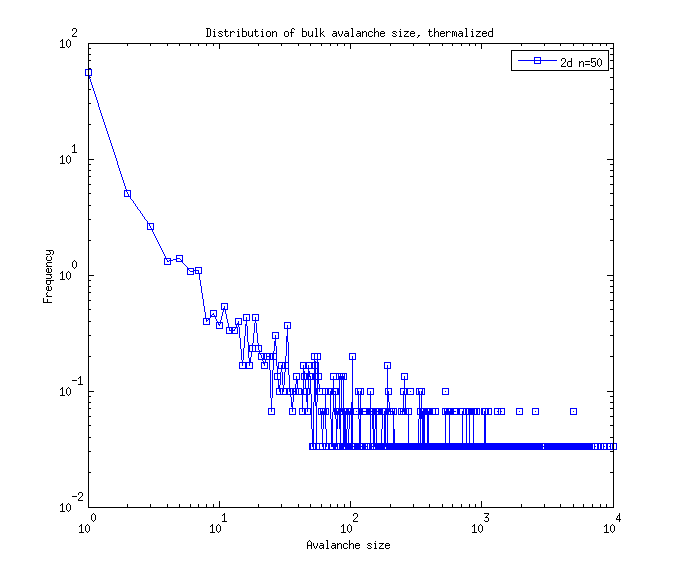
\includegraphics[width=0.49\textwidth]{results/sbulk_th.png} 
\caption{Avalanche size distribution for $50\times50$ lattice. 
The left one shows the result caused by perturbations in site $(1,1)$, namely in the corner; 
and right one shows the result caused by perturbations in a bulk site, $(25,25)$. The driving time is $T=5000$.  }
\label{sv}
\end{center}
\end{figure} 


The relation of the number of sites in the volume respect to the number of sites at boundary should be proportional to $n$, as it is basically the ration of volume and area.
Thi implies that for large lattices, one encounters much more very large avalanche respect to a smaller lattice. For a randomized grain addition, we see similar behaviour as the bulk case.

If we add friction and go to the real case, the number of huge avalanche reduces. Again, we see the importance of friction to modelate the distribution to more a power-law like one.



\subsection{Slowly driven test}
A part from friction, we can also study what happens if we additionally add grain during the avalanche process, let's call this parameter $h$.
We see that the system indeed goes less power-law like.

In mean field theory, one can consider this $h$ parameter as a fine tuning parameter, as when $h\longrightarrow0$, the systems turns to have a better statistics.

However, from our studies, we are less precise and think that the criticality is achieved by an interplay of grain addition and dissipation, with dissipation in average. 

 
\section{Conclusion}

SOC is still a vague phenomenology, that many attempts to use it to explain the many power-like distribution in real systems using computational models.

From the studies of different cases of the abelian sandpile, we conclude that the continuous case, with real field and friction in propagating the grains, 
the system bears nice power-law like distribution for avalanche size, and a bit worse fit for avalanche lifetime. 
This case, independent of the boundary conditions, is also the more realistic one, therefore, one might identify it with SOC. 

In summary, we associate \textbf{slowly driven} systems with \textbf{dissipation} and a \texbg{local threshold} that leads to avalanche phenomena, to SOC, 
and our computational models bear these characteristics. 
Distinct specific laws might change only the critical exponent. 

The cellulla automation models of sandpile is then, a convenient way to modelize real systems with the discussed properties.

A deeper understanding of SOC, if it exists, definitely needs a mathematical framework. 